%Styles
\tikzstyle{ground}=[color=gray,postaction={draw,decorate,decoration={border,angle=-45,amplitude=0.2cm,segment length=2mm}}]
\tikzstyle{cart} = [draw, fill=cyan!10, rectangle, minimum height=1cm, minimum width=1.2cm, rounded corners =0.1cm,node distance=2cm]
\tikzstyle{actuator} = [draw=black ,fill=black!10!white, thick, rectangle, inner sep=0,minimum height=0.6cm, minimum width=0.2cm, node distance=3cm]
\tikzstyle{spring} = [thick,black,decorate,decoration={snake,amplitude=3,segment length=10}]
\tikzstyle{wheel} = [thick,orange,decorate,decoration={coil,aspect=0.7,amplitude=5}]
\tikzstyle{cart} = [rectangle, inner sep=0,minimum height=0.8cm, minimum width=1cm, node distance=3cm, path picture={ 
      \shadedraw[left color=white,right color=gray!40!white, thick] ([yshift=0.12cm, xshift=0.3pt] path picture bounding box.south west) rectangle ([xshift=-0.3pt,yshift=-0.3pt] path picture bounding box.north east); 
      \draw[very thick, fill=white] ([yshift=0.12cm, xshift=0.2cm] path picture bounding box.south west) circle (0.1cm);
      \draw[very thick,fill=white] ([yshift=0.12cm, xshift=-0.2cm] path picture bounding box.south east) circle (0.1cm);}]
\tikzstyle{pt} = [coordinate]
\tikzstyle{force}=[thick,->,>=latex,draw=blue,fill=blue]

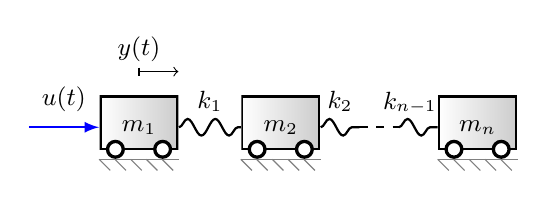
\begin{tikzpicture}[scale=1,every node/.style={font=\small}]

%Nodes
	\node[pt]		(act)					{};
	\node[cart,]	(m1)		[right of=act, node distance=1.4cm]			{$m_1$};
	\node[cart] 	(m2) 		[right of=m1, node distance=1.8cm] 	{$m_2$};
       \node[pt] 	(pt1) 		[right of=m2, node distance=1cm] 	{};
	\node[pt] 	(pt2) 		[right of=pt1, node distance=0.5cm] 	{};
	\node[cart] 	(m3) 		[right of=pt2, node distance=1cm] 	{$m_n$};

%Connections	
	\draw[force] (act) -- node[above, yshift=2pt] {$u(t)$} (m1);
	\draw[spring] (m1) -- node[above, yshift=2pt] {$k_1$} (m2);
	\draw[spring] (m2) -- node[above,yshift=2pt] {$k_2$} (pt1);
	\draw[thick, dashed] (pt1) -- (pt2);
	\draw[spring] (pt2) -- node[above, xshift=-3pt, yshift=1pt] {$k_{n-1}$} (m3);
	
	\draw[ground] (m1.south west) -- (m1.south east);
	\draw[ground] (m2.south west) -- (m2.south east);
	\draw[ground] (m3.south west) -- (m3.south east);
	
	\draw[] ([yshift=0.35cm]m1.north) -- +(0,-0.1cm);
	\draw[->] ([yshift=0.3cm]m1.north) node[above] (A1) {$y(t)$} -- +(0.5cm,0);
	
\end{tikzpicture}
